\documentclass[../../main.tex]{subfiles}

 \lhead{Implementation: Odeon}
 
\begin{document}

\subsection{ODEON}
	\label{odeon}
	\subsubsection{Water Tightness Test}
		Once the the SketchUp model had been exported as a .par file using the SU2Odeon plug-in \cite{SU2Odeon} it could be opened in Odeon and checked to ensure that there were no gaps in the model for which rays to escape. If this was the case, the model would have to be fixed in SketchUp and reimported into Odeon. Odeon makes checking the model easy by running a `\textbf{water tightness}' check where a large number of rays are reflected around the room seeing whether any of them manage to escape. Figure~\ref{watertight} shows the Hendrix Hall model undergoing such test. Once it was ensured that the model was fit for use, the surface materials could be assigned.

		%-------------Water tightness test-------------%
		\begin{figure}[ht]
			\center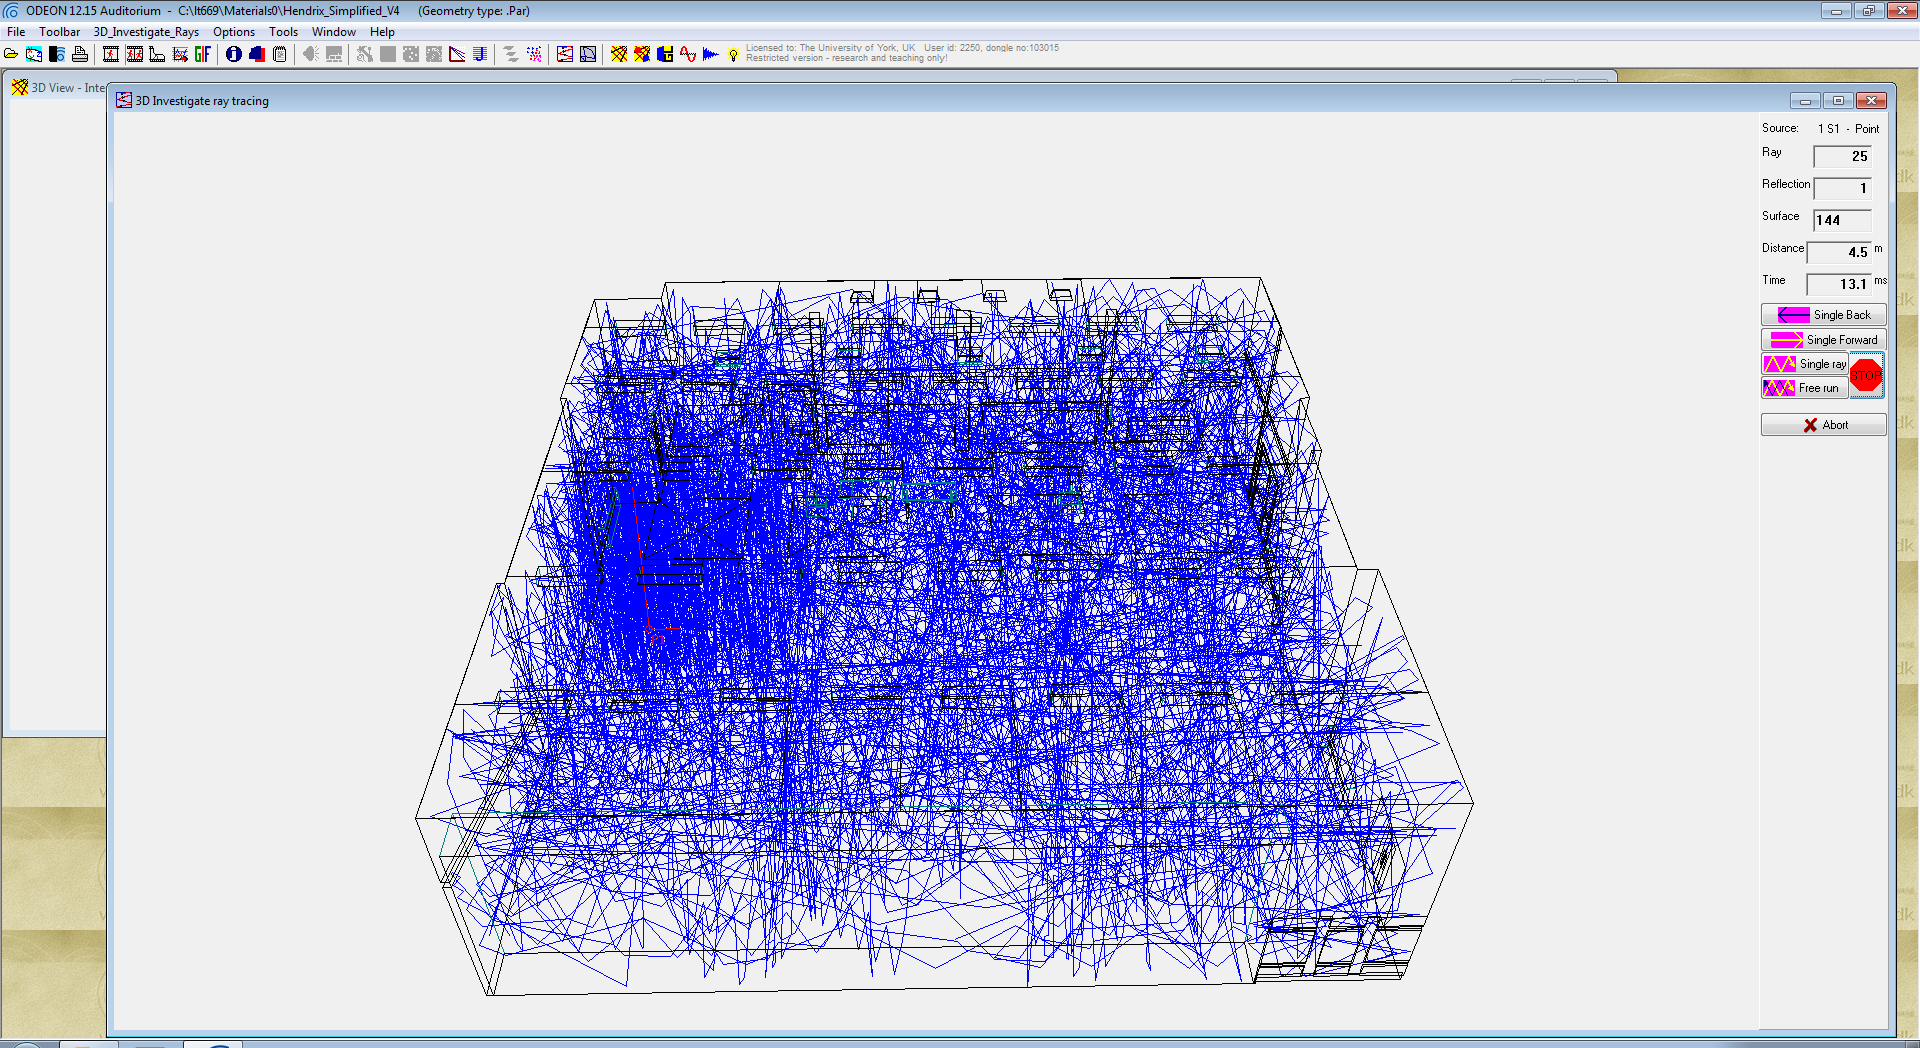
\includegraphics[scale = 0.3]{Sections/Implementation/Odeon/images/OdeonRays/waterTight2.PNG}
			\caption{Hendrix Hall model undergoing a water tightness test in Odeon}
			\label{watertight}
		\end{figure}

	\subsubsection{Material Selection}
	\label{odeon:materials}
		The surface materials within a room have a huge impact on how sound propagates around a room, heavily effecting reverberation time and frequency content of said reverb. It is therefore imperative to assign materials as accurately as possible to produce an accurate representation of a known acoustic environment. For this, Odeon provides a material list of common materials often found when constructing building.

		\paragraph{Initial Materials}
			As the exact surface materials of Hendrix Hall are not known and Odeon's material list was limited to materials that seem to be tailored for construction sites only, assumptions had to be made for the original surface materials. In some cases, appropriate materials were not available therefore new materials had to be added to the material list. This can be done by finding a materials absorption coefficients, selecting `\textbf{Edit an existing material}' where new materials absorption coefficients can be entered and saved as a new material. Required materials that were absent from Odeons material list include:

			\begin{center}
				\begin{tabular}{r l}
					\textbf{Material} & \textbf{Surface applied to} \\ \hline
					Hard Plastic \footnotemark & Roof lights and projector covers \\
					Mineral fibre \footnotemark & Ceiling Tiles \\
					Slate \cite{Kovalchik} & Blackboard \\
				\end{tabular}
			\end{center}

			\footnotetext{Avilable: http://www.acoustic.ua/st/web\_absorption\_data\_eng.pdf}
			\footnotetext{Avilable: http://www.bembook.ibpsa.us/index.php?title=Absorption\_Coefficient\&action=edit}

			 This is shown in figure~\ref{materialEdit}
			 An example of materials is as follows

			 A full material list is available in `\texttt{Material\_List\_V2.xlsx}'

		\paragraph{Surface Types}

			For a number of surfaces it is appropriate to additionally edit properties other than just their absorption coefficients.

			As explained in section \nameref{designRoom}, the roof hangings are constructed of four joint slanting surfaces. To prevent Odeon from calculating the diffraction due to each individual surface, the combination of surfaces can be set to \textbf{Fractional}.

			%-------------Material Edit Image-------------%
			\begin{figure}[ht]
				\center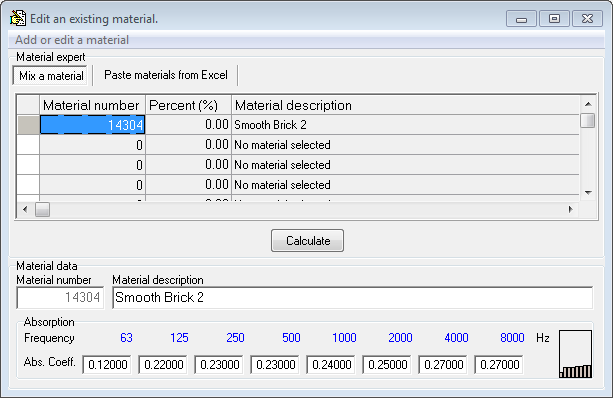
\includegraphics[scale = 1]{Sections/Implementation/Odeon/images/Absorption.PNG}
				\label{materialEdit}
				\caption{Absorption coefficient editing window in Odeon used to add unavailable materials}
			\end{figure}



		\paragraph{RIR Comparison}

		\paragraph{Final Material Choice}

			The incorrect \ac{RIR}'s were used to calculate the room materials to begin with. Upon rendering new \ac{RIR}'s, three tests \ac{RIR}'s were rendered with the three main differences in materials selection in order to check that the spectrogram was close enough to the real \ac{RIR}'s
			\paragraph{Original Material Selection}

	\subsubsection{RIR Outputs}

		\paragraph{RIR Topology Problems}
			%Show original output RIR

			%Show timing errors

			%Show Height Test Images

			%Show new RIRs with correct timings

	\subsubsection{RIR Locations}
	
\end{document}